\section{Dynamic Memory: retaining a reusable answer calculation}
\label{section:memory-as-a-retained-and-reconstructable-object}

A memory is a representation built now to answer questions later. The useful object is not necessarily a compressed paragraph or a list of nearby passages. It may be a small calculation that preserves the relation the question asks about, together with the source records needed to check and revise it. Corpus as a State develops geometric retention and reconstruction. Dynamic Memory develops retained conditional structure, query propagation and source-supported revision. Both are classical constructions.

Consider four source cards. One records a purchase before approval, another a purchase after approval, and two describe unrelated events. A quotation belongs to the original record. An extracted field such as \emph{purchase before approval} is an observation that must be checked against that quotation. A numerical indicator selecting that field is a further construction. Keeping those stages separate tells us what the memory can answer. If the temporal field was never extracted, a larger vector basis cannot manufacture it.

Suppose the first two cards form one group and the other two another. A group average gives the same result whether the selected card is the purchase before approval or the purchase after it. Keeping their internal contrast restores the distinction. This is the same problem as the four-state process: two situations look identical after reduction but require different answers. We first show how geometric and operator retention preserve that contrast, then how a conditional continuation can retain an entire reusable calculation.
The original \emph{Corpus as a State}~\cite{Referencece8431} begins with vectors describing source items. If the rows of $X$ are normalised item vectors, its state-like summary is
\begin{equation}
 \rho=\frac{X^T X}{N},\qquad q^T\rho q=\frac1N\sum_{i=1}^N(x_i^Tq)^2.
 \label{eq:corpus-state}
\end{equation}
Here $N$ is the number of items and $q$ a unit query direction. The quadratic form reports how much of the collection lies along that direction. It does not by itself identify which document supplied the contribution. Source identities and witness records must remain available separately. The quantum-like notation packages familiar covariance and projection geometry into an account of what the collection retains.

For reconstruction, the mean and centred covariance matter. A node can retain a mean $\mu$, an orthonormal local basis $V$ and coordinates along that basis. The discarded covariance eigenvalues quantify mean-square embedding reconstruction error. Parent nodes combine child mass, means and covariance, including both the variation within children and the variation between their means. If a child has already discarded a direction, its error must be carried upwards. Recomputing a small parent residual from truncated children does not recover the lost information.

The original work also gives a certified search rule. Suppose every item in a node has the form $x=\mu+Va+e$, with $e$ orthogonal to $V$, $\|a\|\leq R$ and $\|e\|\leq r$. Then its signed query score satisfies
\begin{equation}
 q^Tx\leq q^T\mu+R\|V^Tq\|+r\|(I-VV^T)q\|.
 \label{eq:search-bound}
\end{equation}
A best-first search may discard a node once this upper bound cannot beat an already found answer. That certificate is different from routing by the nearest centroid. The latter may be fast, but without a bound it is a heuristic. A hierarchy also need not save work: loose bounds can force it to open most nodes, in which case a direct vector scan is preferable.

\subsection{Constructing a source diffusion}
The operator-memory prototype begins with individually identified records and a declared set of questions, not with an operator whose meaning is left to be inferred. In the news example there are 609 articles. A language model reads each article alone and extracts four short fields: object, mechanism, conditions and consequences. Each field has at most thirty words and supporting quotations checked against the article. A frozen encoder maps the fields to 384-component vectors. These descriptions choose the semantic coordinates. The following operator construction describes that earlier prototype, rather than attributing its parameters to every Dynamic Memory enquiry. Conditional on those observations, its numerical steps are explicit.

Consider one field, and write $v_i$ for the unit vector of article $i$. Similarity proposes which records should exchange probability in an auxiliary diffusion. For each article, keep its sixteen nearest neighbours and give a directed edge the nonnegative weight
\[
 h(v_i^Tv_j)=\left(\frac{1+v_i^Tv_j}{2}\right)^2.
\]
Take $a_{ij}=a_{ji}$ to be the larger of the two directed weights, using zero for an absent edge. A record missing this field remains identified but has its incident edges removed. With reference weights $\pi_i=1/609$, define
\begin{equation}
 r_j=\sum_{i\ne j}\frac{a_{ij}}{\pi_j},\qquad
 \kappa=\max\{1,\max_j r_j\},\qquad
 G_{ij}=\frac{a_{ij}}{\kappa\pi_j}\ (i\ne j),\quad
 G_{jj}=-\frac{r_j}{\kappa}.
 \label{eq:memory-generator-construction}
\end{equation}
Column $j$ gives rates out of source $j$. Its entries sum to zero, so total probability is preserved. The symmetric conductance $G_{ij}\pi_j=a_{ij}/\kappa$ gives detailed balance, and the largest exit rate is at most one. This last normalisation fixes the diffusion time used in the tests. In a physical application $G$ can instead be supplied by the actual dynamics. Here it describes a deliberately constructed similarity process on records.

The next step makes this process amenable to spectral compression. Let $p$ be a probability distribution over source IDs, let $W=\mathrm{diag}(\pi)$, and express departures from the reference in weighted coordinates:
\begin{equation}
 y=W^{-1/2}(p-\pi),\qquad L=W^{-1/2}GW^{1/2},\qquad
 A=U^TLU,\quad D=U^TL(I-UU^T).
 \label{eq:memory-object}
\end{equation}
The first transformation gives $\|y\|^2=\sum_i(p_i-\pi_i)^2/\pi_i$. Detailed balance makes $L$ symmetric and nonpositive. Its negative, $H_{\rm mem}=-L$, is the positive dissipation operator: it scores variation across the source graph. The columns of $U$ will specify the retained directions. Once they have been selected, $A$ is the smaller operator acting on retained coordinates, while $D$ measures feedback from the omitted ones.

\subsection{Keeping the internal distinction}
A candidate group of records needs both its total mass and the distinctions within it that a query can resolve. Let $C_{ai}=1$ when source $i$ belongs to proposed group $a$, and zero otherwise. The group masses are $\pi_c=C\pi$. The normalised constant direction for each group is a column of
\[
 U_0=W^{1/2}C^T\mathrm{diag}(\pi_c)^{-1/2},\qquad P_0=U_0U_0^T .
\]
These columns preserve probability assigned to each group. They do not preserve, for example, which of two otherwise similar articles records a purchase before rather than after an approval.

A task vector $f$ assigns a numerical value to each source. A date/source selection can be an indicator, while a field-direction test can be the projection of that article's embedding onto a specified query direction. Its weighted column is $W^{1/2}f$. In the news run, the declared field-direction ensemble gives half its weight to observed source directions and half to differences between each source and its nearest neighbour. These contrast probes make local distinctions part of the demand, rather than asking only for the mean field. Inside each proposed group, remove the constant part and collect the remaining task columns together with columns of $(I-P_0)LU_0$. The latter identify internal variations coupled to the proposed group dynamics. After applying the declared task and dynamics weights, call this local demand matrix $E$.

The leading left singular vectors of $E$, equivalently the leading eigenvectors of $EE^T$, give the rank-limited internal directions $B$. They maximise the retained squared demand at the chosen rank. The resulting map is $U=[U_0,B]$, with orthonormal columns and each internal direction supported within its group. This is a direct linear-algebra calculation, not a further language-model training stage. That prototype gives task and dynamical demands equal family weights, scales the dynamical demand by $0.1$, and permits at most eight internal coordinates per parent. It then checks the actual task losses and the full closure defect. A good spectral approximation proposes a useful memory, while these checks determine whether it is adequate.

The groups themselves are proposals too. Diffusion eigenvectors provide coordinates in which a reproducible clustering routine suggests neighbouring records to combine. The construction accepts a new level only if it reduces the object count and meets its declared error thresholds. At the next level, all retained child coordinates enter the parent calculation, including the internal contrasts. The parent carries the transformed operator, the decoder, exact source membership and the inherited error account. Passing only child averages would throw away the very information the internal coordinates were purchased to retain.

Return to the four source cards. Record 1 marks purchase before approval and record 2 purchase after approval. Put those records in one group and records 3 and 4 in another, with uniform reference $\pi_i=1/4$. The query \emph{before approval} has task vector $f=(1,0,0,0)^T$. Keeping group mass alone maps either source selection $p=(1,0,0,0)^T$ or $p=(0,1,0,0)^T$ to the same reconstruction $\hat p=(1/2,1/2,0,0)^T$, hence the same estimated answer $f^T\hat p=1/2$. Adding the internal contrast $b=(1,-1,0,0)^T/\sqrt2$ to $U$ recovers the exact answers one and zero. The illustration shows what the selected direction buys: the decoder can use a distinction that the source cards and task definition made explicit. If ingestion never records that temporal distinction, choosing a larger numerical basis alone cannot supply its meaning.

With $z=U^TW^{-1/2}(p-\pi)$, the linear reconstruction and task estimate are
\[
 \widehat p=\pi+W^{1/2}Uz,\qquad
 \widehat{f^Tp}=f^T\pi+f^TW^{1/2}Uz.
\]
This reconstructs linear task values. Positivity of every reconstructed probability is a separate constraint.




For the declared task vector $f$, the desired expectation is $f^Tp$. Writing $P_U=UU^T$, the error from discarding the orthogonal fluctuation is bounded by
\begin{equation}
 |\delta(f^Tp)|\leq\|(I-P_U)W^{1/2}f\|\sqrt{\chi^2(p\Vert\pi)}.
 \label{eq:memory-task-error}
\end{equation}
The first factor measures whether the task direction was retained. The second uses the chi-squared divergence $\chi^2(p\Vert\pi)=\sum_i(p_i-\pi_i)^2/\pi_i$ to measure how far the queried distribution moves from the reference. A basis that works near the average collection may be inadequate for a rare conditional slice. This gives refinement a concrete trigger. Under reversible contraction, the corresponding dynamical mismatch has a finite-time bound proportional to $t\|D\|$, and exact elimination again supplies a memory kernel when an autonomous approximation is inadequate.


Figure~\ref{fig:dd-memory-mechanism} follows the two constructions from source items to an answer. In the original route, local geometric summaries support projection and certified search. In Dynamic Memory, retained task/law coordinates and reconstruction travel together. A query selects a task or source-conditioned distribution, the decoder computes the requested quantity, and a residual or capacity failure can send the calculation back to finer records. A language model may compose a final response from returned witnesses, but its prose is not the same object as the numerical decoder.
\begin{figure}[htbp]
\centering
\small
\begin{tabular}{p{0.44\linewidth}p{0.44\linewidth}}
\hline
\textbf{Geometric retention} & \textbf{Retained query calculation}\\
Located source records & Located source contributions\\
$\downarrow$ field vectors & $\downarrow$ joint observations\\
Local means and basis directions & Conditional continuation states\\
$\downarrow$ task projection and bounds & $\downarrow$ forward or adjoint messages\\
Reconstructed task value & Joint mass or conditional answer\\
$\downarrow$ source refinement when needed & $\downarrow$ affected paths revised on edit\\
\hline
\end{tabular}
\caption{Two retained objects for different enquiries. A local geometric basis preserves specified variations among records. A conditional continuation shares equal future calculations while retaining source incidence separately. Both need an observation step before numerical retention and a witness route after it. A language reader composes an answer from delivered evidence, rather than replacing the decoder or the source check. This is an explanatory schematic, not a performance comparison.}
\label{fig:dd-memory-mechanism}
\end{figure}

\FloatBarrier
\subsection{A shared conditional continuation}
Retaining a few directions is useful when the question concerns variation among vectors. When the records instead contain discrete fields and the query asks for a joint condition, we can retain the rule connecting those fields directly. This categorical route starts from weighted records of discrete fields, written $(x_1,\ldots,x_d)$ in a fixed field order. A \emph{prefix} is the part already read, and a \emph{suffix} is the part still to come. Two prefixes can share one continuation state when they imply exactly the same conditional probability law for every suffix. Build the representation backwards from the terminal field, merging equal normalised continuations. Each edge stores the probability of the next symbol and its successor state. Source IDs remain accessible as witnesses rather than being inserted as extra random fields that would prevent useful merging.

A query supplies a factor $q_g(x_g)$ at field $g$. For a Boolean filter it is one for an allowed value and zero otherwise. An unqueried field uses one for every value. If state $s$ at level $g$ takes symbol $a$ with probability $t_g(s,a)$ and proceeds to state $b(s,a)$, its answer is the backward message
\begin{equation}
 m_s=\sum_a t_g(s,a)\,q_g(a)\,m_{b(s,a)},\qquad m_{\rm terminal}=1.
 \label{eq:memory-continuation-message}
\end{equation}
The root message is the probability of satisfying the whole query. This recursion keeps joint constraints because the successor depends on the preceding symbols. Replacing the joint law by separate field averages would remove that dependence. For integer empirical weights, the implemented Boolean lane stores primitive denominators and integer edge multipliers instead. Checked integer messages give exact counts and refuse a requested arithmetic width that would overflow.

This also explains the tensor-network connection without requiring a quantum device. Putting $\sqrt{t_g(s,a)}$ on the corresponding local transition gives a product of tensors whose amplitude for a complete record is $\sqrt{p(x_1,\ldots,x_d)}$. Contracting the amplitude tensors with their conjugates and the diagonal query factors computes the same probability, $\sum_x p(x)\prod_g q_g(x_g)$. Singular-value decompositions can compress this representation when approximation is allowed, with the final contracted error checked separately. Figure~\ref{fig:dd-memory-parity} benchmarks exact categorical messages, while Eq.~\eqref{eq:memory-object} describes the source-diffusion route. They are alternative retained objects for different input and query interfaces.~\cite{Referencea10bf0}

The parity relation makes the messages tangible. Consider four equally likely three-bit records: $000$, $011$, $101$ and $110$. Every individual bit is balanced and every pair looks independent, yet the third bit is determined by the first two: it is their exclusive-or. Marginal summaries lose that rule. A two-state continuation that records even or odd parity preserves it. Extending the construction to $d$ bits gives $2^{d-1}$ distinct records but still only two continuation states. After reading a bit, the continuation either keeps its even/odd state for zero or flips it for one. At the last field, only the value that finishes with even parity is allowed. For instance, the prefix $01$ requires the last bit to be $1$, while $00$ requires $0$. The same two states can be reused at every level. Compactness comes from this composable rule, not from many identical rows.


\subsection{Propagate the question through the retained relation}
\label{subsec:dynamic-propagator}

The backward message in Eq.~\eqref{eq:memory-continuation-message} is one way to perform the query. Dynamic Memory also expresses it as a forward propagator. This makes the connection between a source observation, a retained law and an answer explicit.~\cite{Referencea10bf0,McCaul2026164581} At field position $g$, let $a$ label the current continuation state, $b$ a successor, $x$ a possible category and $\delta_g(a,x)$ its deterministic successor. For a filter $0\leq f_g(x)\leq1$, define
\begin{equation}
 M_g^f[b,a]=\sum_{x:\delta_g(a,x)=b}t_g(a,x)f_g(x).
 \label{eq:dynamic-query-matrix}
\end{equation}
Each column describes how mass at a current state passes to the next field. Without a filter its sum is one. With a filter it is at most one: rejected possibilities lose mass. If $v_0$ places unit mass at the root, the final mass is
\begin{equation}
 Z(f)=\mathbf1^{\mathsf T}M_{d-1}^f\cdots M_0^f v_0
     =\sum_xp(x)\prod_{g=0}^{d-1}f_g(x_g).
 \label{eq:dynamic-query-mass}
\end{equation}
Here $d$ is the number of ordered fields and $\mathbf1$ sums the terminal masses. The equality follows by expanding the paths: their conditional probabilities multiply to the joint probability $p(x)$. Backward messages evaluate the same contraction in the opposite direction. They reuse a common suffix calculation whenever two prefixes induce the same future law. An unfiltered suffix has message one and can be skipped.

This propagator has a literal selective-channel representation, conditional on the stated positive filters. The matrices
\[
 K_{bax}=\sqrt{t_g(a,x)f_g(x)}\,|b\rangle\langle a|
\]
define the map $\rho\mapsto\sum_{b,a,x}K_{bax}\rho K_{bax}^{\dagger}$. Its diagonal populations follow $M_g^f$, and
\[
 \sum_{b,a,x}K_{bax}^{\dagger}K_{bax}
 =\sum_a\left[\sum_x t_g(a,x)f_g(x)\right]|a\rangle\langle a|\leq I .
\]
Thus the map preserves positivity even when applied to part of a larger state, and cannot increase total trace. This is what \emph{completely positive, trace-nonincreasing} means here. The extension removes input coherences. It represents a classical filtering calculation in operator language, rather than assuming a quantum implementation. Normalising a selected result requires positive surviving mass. Signed query factors need a different interpretation.

The two indices in this account have different meanings. The field index $g$ orders a finite query calculation. The time $t$ in Eq.~\eqref{eq:general-memory} evolves a declared source process or an auxiliary diffusion. For the reversible operator $L$ of Eq.~\eqref{eq:memory-object}, write $Q_U=I-UU^T$, $\eta(0)=Q_Uy(0)$ and $L_Q=Q_ULQ_U$ on the omitted space. Exact elimination gives
\begin{equation}
 \dot z(t)=Az(t)+D e^{tL_Q}\eta(0)
 +\int_0^t D e^{(t-s)L_Q}D^Tz(s)\,ds .
 \label{eq:dynamic-reduced-memory}
\end{equation}
Symmetry of $L$ supplies the transpose in the kernel. The formula says what an autonomous retained evolution leaves out: initial hidden state and feedback through hidden modes. A small query graph and a closed dynamical reduction are separate achievements. Connecting them requires a specified evolution and preparation, not merely calling both a propagator.

\subsection{Revise the calculation when a source changes}
\label{subsec:dynamic-updates}

A reusable answer must also survive corrections. Let $A$ label a population and $B$ an event. Four distinct source batches contribute joint counts $(n_{00},n_{01},n_{10},n_{11})=(4,1,1,4)$ in tuple order $(A,B)$. The requested fraction is
\[
 P(B=0\mid A=0)=\frac{n_{00}}{n_{00}+n_{01}}=\frac45.
\]
Correct the first batch from four to three, add a distinct batch at $(0,1)$, then withdraw the old batch at that tuple. Figure~\ref{fig:dynamic-witnessed-update} shows the successive answers. The identity of the withdrawn batch matters even though two batches have identical field values.

\begin{figure}[htbp]
\centering
\small
\begin{tabular}{p{0.32\linewidth}cccc}
\hline
Source operation & $n_{00}$ & $n_{01}$ & Selected mass & Answer\\
\hline
Initial observations & 4 & 1 & $5/10$ & $4/5$\\
Correct first batch & 3 & 1 & $4/9$ & $3/4$\\
Add a distinct batch & 3 & 2 & $5/10$ & $3/5$\\
Withdraw the old batch & 3 & 1 & $4/9$ & $3/4$\\
\hline
\end{tabular}

\vspace{0.8em}
\fbox{\parbox{0.88\linewidth}{\centering
Located source revision $\;\longrightarrow\;$ joint count change\\[3pt]
$\longrightarrow$ affected prefix path $\longrightarrow$ revised conditional message\\[3pt]
$\longrightarrow$ joint mass divided by conditioning mass}}
\caption{A witnessed answer update. The other population keeps counts $(1,4)$ throughout. After correction, root mass $4/9$ for $A=0$ times suffix message $3/4$ for $B=0$ gives joint mass $1/3$. Dividing by $4/9$ recovers $3/4$. The $A=1$ conditional suffix is unchanged even when its root weight changes. The table is the exact arithmetic of the stated construction, not a timing experiment or independent validation of the update implementation.}
\label{fig:dynamic-witnessed-update}
\end{figure}

The representation therefore retains unmerged prefix counts and source incidence beside the shared continuation states. An edit retracts the old contribution, admits the new source revision, and copies the affected prefix path. It recomputes rational transition probabilities and successor signatures there. Equal signatures share one continuation again. Query bindings on affected ancestors are invalidated, while messages on unchanged immutable signatures remain reusable.

Keeping the unmerged occurrences is essential. Counts $(3,1)$ and $(12,4)$ induce the same conditional law $(3/4,1/4)$, so they can share a future calculation. Changing the latter to $(8,4)$ splits the laws. The retained source-labelled occurrence says which use must change. Sharing a calculation need not merge the evidence that may later make its uses diverge. If conditioning support becomes zero, the conditional answer is undefined, rather than zero.

\subsection{Which size controls the saving?}

Let $S_g$ be the number of continuation states at field $g$ and $c_g$ the number of categories. Dense transition storage uses $O(\sum_gS_gc_g)$ slots, beside source and witness storage. For $Q$ queries, let $A_g\leq Q$ remain active after zero-filter and unfiltered-suffix shortcuts. Evaluation uses
\begin{equation}
 O\!\left(\sum_g A_gS_gc_g\right)
 \label{eq:dynamic-query-cost}
\end{equation}
arithmetic slots, or the visited edges for a sparse implementation. Direct scanning instead tests the relevant factors on the records, costing $O(QNd)$ elementary factor work before packed-word improvements. The parity example is favourable because $N=2^{d-1}$ while each cut has only two continuations. A general law can require almost its entire prefix trie. Field order, repeated conditional structure and query support determine the saving.

One changed tuple touches at most $d+1$ raw prefix nodes. With bounded category count $c$, copying outgoing slots and hashing local signatures takes $O(dc)$ slot work, in addition to parsing, dictionary access and rational arithmetic. Recomputed messages must be charged to their affected dependency cone. Multiple tuple changes or a changed field order can make that cone broad. Returning $k$ witnesses also requires at least $O(k)$ output work, regardless of how cheaply a count was obtained.

These propagator and update constructions are central proposals in Dynamic Memory. Their finite equations are explicit, and the source describes a small exact-arithmetic update fixture. Independent scientific verification of that implementation and its scaling remains pending. The older measured comparison below concerns already-built exact continuations on a particular parity/query family. It does not measure incremental source updates or establish a general semantic-memory advantage.

The exact-query campaign implements this continuation rule with checked integer arithmetic, Boolean product queries and source witnesses. Figure~\ref{fig:dd-memory-parity} shows its warm-query advantage over the two recorded scans for the 19-bit law. Construction is paid separately, so the useful workload consists of repeated queries on an already built representation. The controls explain when that economy changes: arithmetic-width limits trigger an explicit refusal, and a weighted scan wins on duplicate-heavy data. In the displayed timing family every query fixes four prefix bits and therefore has exactly $2^{14}=16{,}384$ matching worlds. A sixteen-entry prefix-count table could answer that restricted family too. Comparisons against exact indexed alternatives and queries involving the high-order relation are consequently the next test.
\begin{figure}[htbp]
\centering
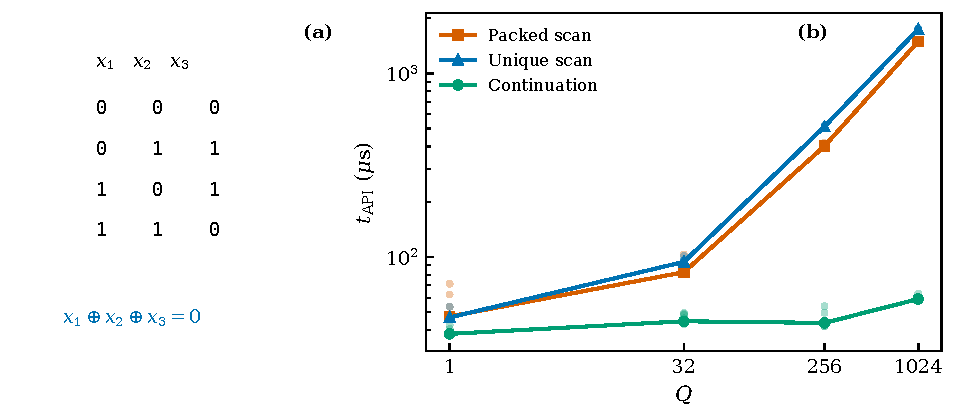
\includegraphics[width=\linewidth]{figures/portable-run-b69220b3a27348ad.result/dd-memory-parity.pdf}
\caption{Retain the relation rather than its list of instances. (a) In the uniform three-bit even-parity law, each pair is independent but two bits determine the third. A running parity state represents the allowed continuations. (b) Archived timings for the 19-bit law with 262,144 distinct worlds, queries fixing four prefix coordinates and batch size $Q$. All displayed prefix queries have count 16,384. The plotted $t_{\rm API}$ is warm full-API time per batch. Dots are all eleven samples and lines join medians. Build, query preparation and first-process compilation are excluded. The campaign also records capacity refusals and a duplicate-heavy control in which direct scan wins.}
\label{fig:dd-memory-parity}
\end{figure}

\subsection{What the language comparisons establish}
The language campaigns test a longer chain: extracting source descriptions, choosing evidence and composing an answer with a language model. Their controls keep those stages distinguishable. In the news experiment, 609 articles supply a 48-question held-out MultiHop slice. At a 2,000-token evidence budget, Parallax answers 40 questions correctly, flat retrieval 39 and the RAPTOR implementation 35. The comparison called the \emph{metadata control} also answers 40. This is a deliberately simpler readout of the same ingested collection: it uses the same original passages, frozen passage embeddings, source identities and publication dates. The same query compiler separates the question into facets and applies any explicit source/date constraints. It then scores every passage directly by the query--passage inner product, selects up to twenty candidates per facet, and uses the common 2,000-token context packing and reader. It bypasses the semantic cards and the hierarchical representation. Thus the control measures what the shared ingestion and flat, condition-aware retrieval already achieve. The comparison holds Atlas's shared ingestion and conditional retrieval stages fixed. All 48 resulting contexts are byte-identical to Parallax's. For this query family the corrected method successfully preserves the same fine-passage target, while the accuracy result leaves the value of its different internal execution to be assessed through cost and scaling.

The QASPER scientific-paper question-answering test covers 256 questions, of which 235 have positive evidence. At a 4,000-token budget, memory and dense retrieval both cover 182 of those 235 questions, compared with 179 for hybrid and 171 for lexical retrieval. Memory and dense retrieval return identical contexts for 252 of the 256 questions. Here the memory route largely reproduces the dense baseline. These are evidence-coverage counts, distinct from the accuracy of the reader's final answer.

LongMem provides a sharper test of relations across a conversational history. With the same reader and a 4,000-token evidence budget, the memory implementation trails dense and hybrid retrieval both in evidence coverage and in final answers. Figure~\ref{fig:dd-memory-reader-controls} shows the answer counts for all 48 questions and the nine-question temporal subset. The weakness falls on precisely the relations and ordering questions that motivate a richer retained representation.
\begin{figure}[htbp]
\centering
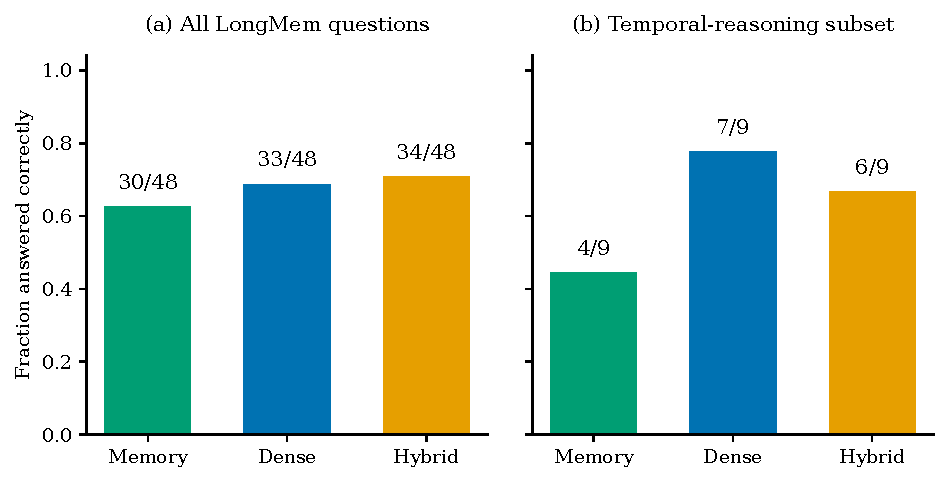
\includegraphics[width=\linewidth]{figures/completion-run-7bd75062068b432b.result/dd-memory-reader-controls.pdf}
\caption{Where the language-memory implementation needs improvement. Archived LongMem answer counts with the same reader and a 4,000-token evidence budget. Memory, dense and hybrid retrieval answer 30, 33 and 34 of the 48 questions correctly. On the nine temporal questions the counts are 4, 7 and 6. The small temporal subset identifies concrete failures to investigate, rather than estimating a universal performance gap.}
\label{fig:dd-memory-reader-controls}
\end{figure}

\subsection{The missing relation and the missing passage}
A source-level audit separates two mechanisms. One development question asks how many projects a person has led or is currently leading. All four required turns are present among the 505 source records, but whole-question embedding retrieval ranks them 63rd, 111th, 208th and 228th. Combining parent and child queries changes those ranks to 66th, 112th, 207th and 241st. Neither the 2,000- nor the 4,000-token context contains the required evidence. The data exists. What is missing is an effective translation from the question to a join over project identities, leadership roles and time, followed by a count. A parent embedding alone does not supply that operation.

A purchase-order question fails differently. Its two support records rank first and ninth under the whole question, and first and seventeenth after merging. Both enter the 2,000-token context, but a first-fit packing rule admits earlier, larger groups at 4,000 tokens and displaces a needed later record. More nominal space can therefore produce a worse evidence set. This is a packing defect, distinguishable from failure to encode a relation during ingestion.

Doubling the evidence budget in the follow-up improves all three methods and helps memory on multi-session questions. Some contexts nevertheless lose previously selected evidence when the budget grows. The audit therefore identifies two different improvements: represent the missing relations explicitly and make evidence packing preserve useful support as capacity increases.

The next implementation should therefore make the relation-bearing part of ingestion explicit. Source-backed entity identities, aliases, roles, events and temporal qualifiers would give a query something on which to execute a join, count or ordering operation. The test is whether this improves held-out relational answers at a fixed evidence budget, with each answer still traceable to its records. A separate branch-preserving packing test should require that enlarging the budget does not discard already selected support. These proposals turn the audit into tests of relation extraction, query execution and evidence packing.

The exact-coordinate campaign and the language campaign now fit together. The former gives an exact composable construction and a measured advantage over scans on the displayed query family. The latter shows the cost of not yet extracting or accessing the right relation reliably. Together they make memory a practical development target: retain the structure that answers the question, preserve its witnesses, and measure the failures that tell us what to ingest next.

The nearest comparisons already exploit structure. GraphRAG extracts entities and relations with a language model, forms graph communities and writes multilevel community summaries. Queries map over summaries and combine intermediate answers. Its principal evidence concerns global sensemaking over large corpora, including breadth and diversity judged against vector retrieval. It is not merely a cosine index. What it does not supply is the particular operator-intertwining residual and task-error contract in Eqs.~\eqref{eq:memory-object}--\eqref{eq:memory-task-error}. Whether that additional contract helps depends on a task for which it can be evaluated.\footnote{D. Edge et al., \emph{From Local to Global: A GraphRAG Approach to Query-Focused Summarization}, \href{https://arxiv.org/abs/2404.16130}{arXiv:2404.16130}, version 2.}~\cite{Edge202448436b}

RAPTOR recursively embeds, clusters and summarises text, retaining original chunks alongside higher-level descriptions. Its main evaluated retrieval method searches across all levels rather than relying on a logarithmic tree descent. Its results therefore support the value of multiscale representational content, not an automatic routing complexity advantage. The relevant comparison keeps the reader, context budget and evaluator fixed.~\cite{Sarthi2024a1f229}

Retrieval-Centric Deep Learning in Growing Nonparametric Neural Networks~\cite{Reference2026d462c2} supplies another useful comparison. For a linear layer trained by gradient descent,
\[
 W_T=W_0+\sum_{t=1}^T v_tx_t^T,\qquad
 W_Tq=W_0q+\sum_{t=1}^T v_t(x_t^Tq).
\]
Here $W_0$ is the initial weight matrix, $x_t$ the input at update $t$, $v_t$ the negative learning-rate-scaled gradient with respect to the layer output, and $q$ a new input. The stored weight change and the retained input--update pairs give exactly the same linear prediction. The second performs attention-like retrieval over a training history. Kernel constructions extend the connection by evaluating feature inner products without explicitly constructing all feature coordinates. The retained history can still grow with training. The duality reveals an alternative computation, while compression asks which part of that history the future task actually needs.

The useful application is not restricted to conversational recall. Repeated relational enquiries, exception-sensitive corpus inspection and local predictive models all need a representation that preserves more than an average embedding. A memory system becomes more valuable when its answer includes a route back to the source and a meaningful account of what its compression could have missed.

